\chapter{相关理论与方法}
\label{chapter:related-work}
本章将对混合神经隐式场相关理论和方法进行简要的介绍。在\ref{sec: related-work implicit scene representation learning}节中将介绍以神经辐射场\cite{mildenhall_nerf_2020}为代表的使用隐式函数进行场景表示学习的主流方法。纵观神经隐式场发展的历程,人们用来学习场景外观的地图表示方法经历了从纯隐式的多层感知机地图到半隐式的体素地图、低维张量地图的变革,在该节中将详细介绍这一变换的过程和内在原因。在\ref{sec: related-work realistic rendering}一节中,将介绍人们基于神经辐射场上为了使渲染更具真实感所提出的一系列方法,包括引入无界场景压缩、前后景分割等。在\ref{sec: related-work density-distance fields}一节中,我们将介绍辐射-距离混合场景表示的方法。在该节中,我们将首先分析单纯使用辐射场同时表示场景几何和外观所带来的二义性问题,接着从采样策略、体渲染方法、多元传感信息融合以及模型优化几个角度分别介绍相关理论。

\section{神经隐式场景表示学习}
\label{sec: related-work implicit scene representation learning}

神经隐式场景表示,即是将三维场景的几何、外观、语义等信息抽象为一个隐式表示的函数,通过神经网络的回归能力来拟合这些隐函数。在本节中,我们将介绍使用以神经辐射场和神经符号距离场为主的神经隐式表征进行场景表示学习的主要方法。在\ref{sec: related-work MLP-based neural implicit representations}节,我们将通过神经辐射场和DeepSDF介绍使用多层感知机表示场景隐式函数的基本概念,在\ref{sec: related-work grid-based implicit representations}节中介绍神经隐式场景表示的主干模型的改进。


\subsection{基于多层感知机的场景表示}
\label{sec: related-work MLP-based neural implicit representations}

在2020年,Ben Mildenhall等人在ECCV 2020会议上发表了神经辐射场\cite{mildenhall_nerf_2020}(NeRF)用来解决新视角合成任务(如图\ref{fig:related-work novel-view-synthesis-task}所示)。新视角合成任务输入为已知位姿的多视角图片$\{{I}_i\}^N$,希望在该场景的任意给定新视角下,渲染一张具有真实感的图片${I}_\text{target}$。所谓神经辐射场,即是在假设三维空间中任意一个三维点均在向外辐射光线并阻挡其他光线的传播这一前提下,使用一个隐式神经网络建模每个三维点的辐射量。

\begin{figure}[ht]
    \centering
    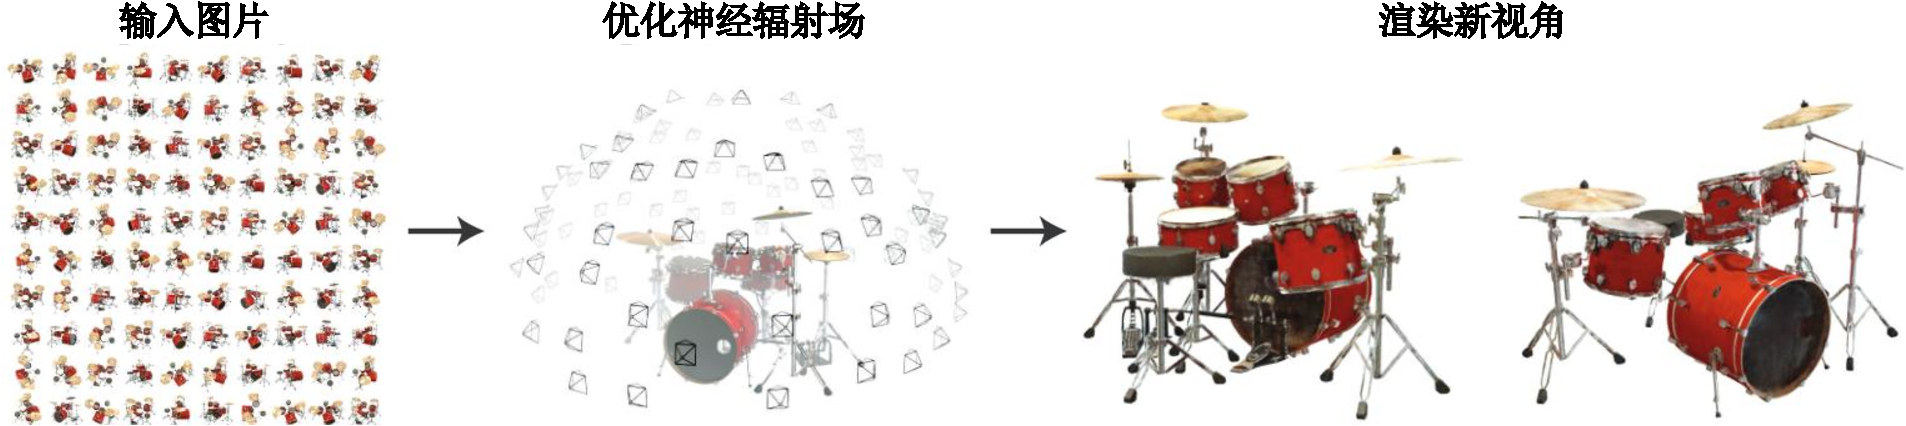
\includegraphics[width=\textwidth]{undergraduate-thesis/images/related-work/NeRF setting.pdf}
    \caption{使用神经辐射场\cite{mildenhall_nerf_2020}进行新视角合成的基本流程}
    \label{fig:related-work novel-view-synthesis-task}
\end{figure}

具体来说,辐射场可以表达为一个输入为三维欧氏空间下坐标$(x,y,z)$和观察角度$(\theta,\phi)$,输出为RGB颜色值$(R,G,B)$和体密度$\sigma$的函数,如公式\ref{eq:related-work radiance field}所示,其中$(x,y,z)\in\mathbb{R}^3, (\theta,\phi)\in[0, 2\pi]^2, \mathbf{c}=(R,G,B)\in[0,255]^3, \sigma\in\mathbb{R}^+$。RGB色值为空间点向外辐射的光的颜色,为了建模高光等物理光照现象,这个值应随观察角度的变化而变化,即$f_{\{R,G,B\}}:f_{\{R,G,B\}}(x,y,z,\theta,\phi)$,相反,体密度$\sigma$只建模三维点的物理密度,是空间点坐标的函数,与观察视角无关,即$\sigma:\sigma(x,y,z)$。根据万能近似定理\cite{hornik_multilayer_1989}(Universal Approximation Theorem),NeRF使用一个多层感知机来建模这种隐式的函数关系,即神经辐射场。
\begin{equation}
    f_\text{NeRF}: (x,y,z,\theta,\phi)\to(R,G,B,\sigma).
    \label{eq:related-work radiance field}
\end{equation}

通过累计一条光线上三维点的辐射值,我们便可以实现在任意观察视角下光线的渲染。图\ref{fig:related-work NeRF pipeline}展示了NeRF方法的总体流程:
\begin{enumerate}
    \item [a] 在观察视角发射一条光线,并在其上采样若干个三维空间点,将他们的三维欧式坐标和观察角度组成一个5元组张量$(x_i,y_i,z_i,\theta,\phi)$;
    \item [b] 通过神经辐射场,得到采样点的隐函数值$(R_i,G_i,B_i,\sigma_i)$;
    \item [c] 使用体积渲染公式,计算整条光线的渲染颜色值$\hat{c}$;
    \item [d] 将渲染值$\hat{c}$与真实观测值${c}_{gt}$比较,计算损失函数,通过反向传播优化神经网络。
    \begin{align}
    c(\mathbf{o},\mathbf{d}) &= \int_0^\infty \sigma(\mathbf{o}+t\mathbf{d})T(t)c(\mathbf{o}+t\mathbf{d},\mathbf{d})\text{d}t,\label{eq: related-work volume rendering}
    \\
    T(t) &= \exp(-\int_0^t\sigma(\mathbf{o}+t\mathbf{d})\text{d}t).\label{eq: related-work transmittance}
    \end{align}
\end{enumerate}


体渲染公式如公式\ref{eq: related-work volume rendering}所示,其中$T(t)$为累计的透光度,如公式\ref{eq: related-work transmittance}所示,通过体渲染,可以将三维辐射场的场景信息投影到二维的成像平面上,进行真实感的渲染。


\begin{figure}[t]
    \centering
    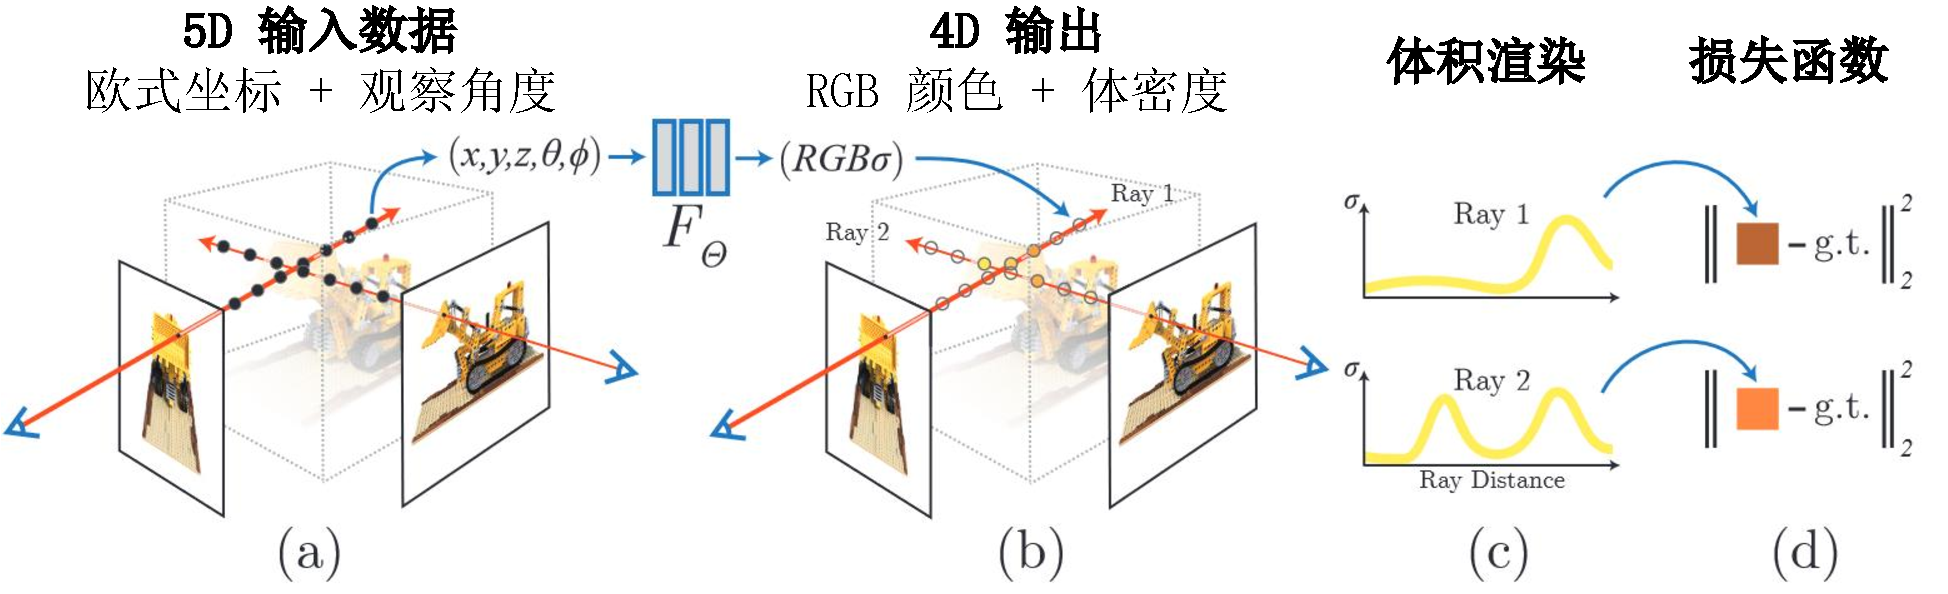
\includegraphics[width=\textwidth]{undergraduate-thesis/images/related-work/NeRF method.pdf}
    \caption{使用神经辐射场\cite{mildenhall_nerf_2020}进行训练和渲染的总体流程}
    \label{fig:related-work NeRF pipeline}
\end{figure}

\begin{figure}[ht]
    \centering
    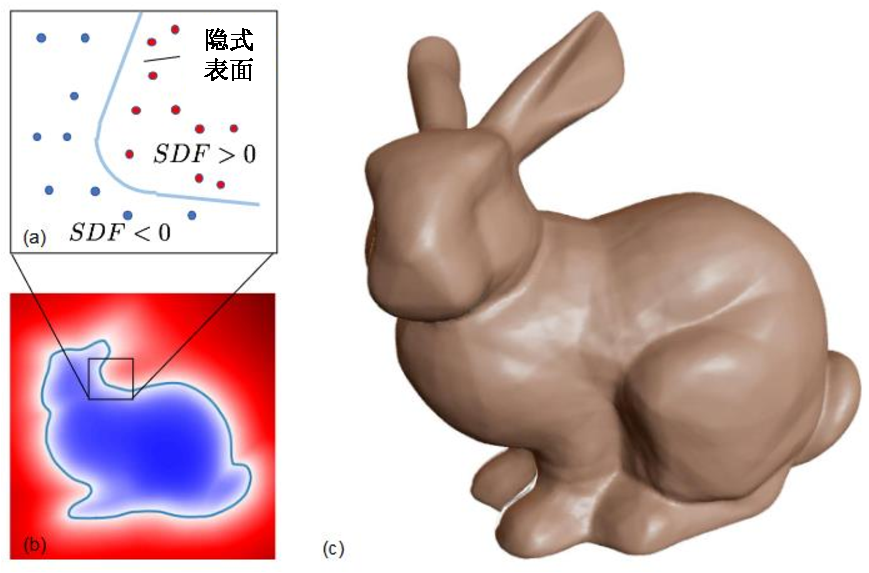
\includegraphics[width=0.7\textwidth]{undergraduate-thesis/images/related-work/SDF concept.pdf}
    \caption{符号距离场示例。图中(a)展示了由SDF函数所隐式确定的表面;(b)为符号距离场在二维的分布,蓝色区域表示SDF<0的区域,红色区域表示SDF>0的区域;(c)由三维符号距离场所确定的几何信息进一步导出的物体模型。}
    \label{fig:related-work SDF concept}
\end{figure}

除了辐射场中的函数关系,基于多层感知机的神经隐式表达也可以被用于其他任务的实现上\cite{park_deepsdf_2019, mescheder_occupancy_2019, shim_snerl_2023, zhi_-place_2021}。2019年Park等人使用多层感知机来拟合场景的三维符号距离场上。符号距离场(Signed Distance Fields, SDF)描述了场景中三维点到物体表面距离,用一个隐式函数$f_{SDF}$表示,如图\ref{fig:related-work SDF concept}所示,有向距离值的绝对值表示某三维点$\mathbf{x}(x,y,z)$到其最近表面的距离,其符号表示三维点在表面内/外,当三维点位于一个封闭曲面内部,则其$f_{SDF}(\mathbf{x}) < 0$,在表面外时$f_{SDF}(\mathbf{x}) > 0$。因此$f_{SDF}(\mathbf{x})$的零值面即为所描述的三维曲面。在DeepSDF中,作者使用一个多层感知机来拟合这一隐式函数。

\begin{figure}[ht]
    \centering
    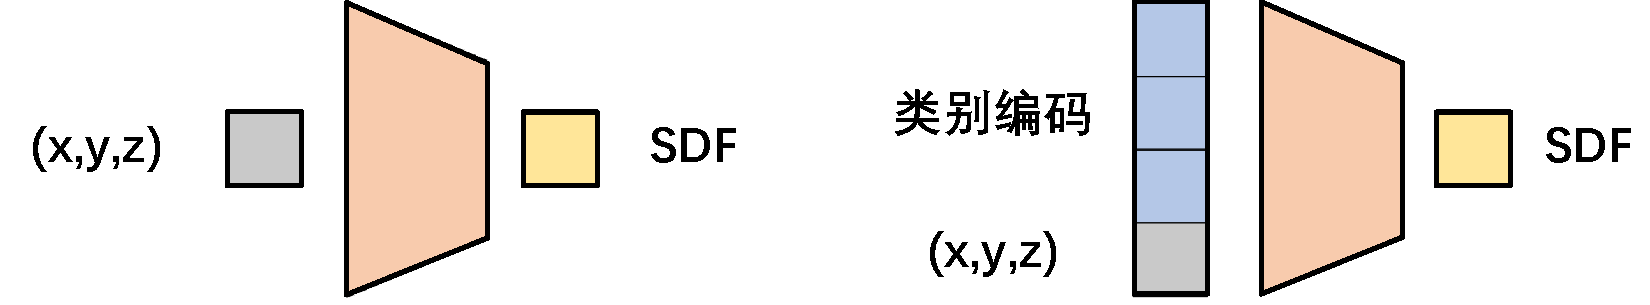
\includegraphics[width=0.8\textwidth]{undergraduate-thesis/images/related-work/deepSDF.pdf}
    \caption{DeepSDF\cite{park_deepsdf_2019}网络结构的两种形式:左侧为一般情形下直接拟合物体的SDF隐函数;右侧是带有类别编码的SDF函数。}
    \label{fig:related-work DeepSDF}
\end{figure}

不同于神经辐射场直接使用多层感知机拟合场景隐函数,DeepSDF引入类别编码,为一类具有相似形状的物体学习类别表征编码,与隐函数输入同时输入网络。这样做可以大大缩减学习同类物体SDF网络的时间,网络结构如图\ref{fig:related-work DeepSDF}所示。



\subsection{基于张量的场景表示}
\label{sec: related-work grid-based implicit representations}
虽然多层感知机作为一个万能函数拟合器在理论上可以无限接近场景的隐式表征函数,但这样的表示主干网络在实践中存在若干问题:
\begin{enumerate}
    \item 多层感知机的训练需要较大计算量,即使训练一个较小物体或场景的隐式函数也往往需要1$\sim$2天的训练时间才能使网络收敛,前向传播的耗时也不能满足计算机图形学实时渲染的需求;
    \item 多层感知机的训练存在遗忘问题。在一组数据上训练产生的梯度往往会影响其他数据上已经收敛的模型权重,这导致以多层感知机为主干网络的模型往往不能泛化到更大的场景上(如完整的室内场景等)。
\end{enumerate}

基于这样的观察,研究者尝试使用基于体素的场景地图主干网络。基于体素网格的场景表示可以采用一种更加直观的方式来表示3D场景,即将3D场景划分为一个网格,并在每个网格内记录它的辐射、法向量等信息。与基于多层感知机的场景表示相比,在训练和前向传播方面,基于体素网格的方法具训练时间短、效果更好等特点。

\subsubsection{传统密集体素网格地图}
早期使用体素网格地图表示的方法\cite{fridovich-keil_plenoxels_2022, kondo_vaxnerf_2021, yu_monosdf_2022}通常将三维场景离散化为一个三维空间网格,其中的每个体素(Voxel)的每个节点上存储该点上的隐式函数值。当需要查询任意一个连续空间中的三维点的隐函数值时,只需查询其周围的八个相邻节点,并使用三线性插值计算目标点的隐函数值。

若用$\mathcal{G}_\theta$来表示一个分辨率为$R_H\times R_W\times R_D$的体素网格,则使用体素网格来作为隐式场骨干模型的方法可以写作:
\begin{equation}
    \hat{s} = \mathtt{interp}(\mathbf{x}, \mathcal{G}_\theta),
\end{equation}
其中$\hat{s}$为网络预测的隐式函数值,$\mathtt{interp}$表示三线性插值。

然而,将三维网格应用于取代原始NeRF中多层感知机的一个必然结果就是对于输入数据的限制。具体而言,原始NeRF使用物体的三维位置坐标和观察角度作为输入来建模物体的Lambertian和非Lambertian效应(即漫反射、高光等与视角相关的效应),然而使用三维网格来建模物体的辐射量则限制了输入维度仅能为三维。这种限制在某些场景下可能会对建模效果产生一定影响。

\begin{figure}[ht]
    \centering
    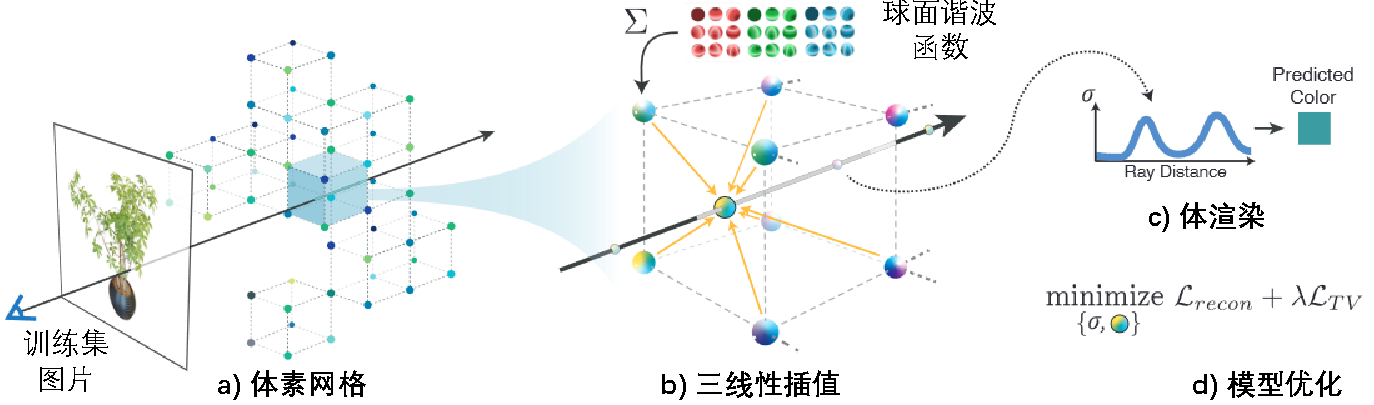
\includegraphics[width=\textwidth]{undergraduate-thesis/images/related-work/plenoxels.pdf}
    \caption{Plenoxels\cite{fridovich-keil_plenoxels_2022} 方法流程图}
    \label{fig:related-work plenoxels pipeline}
\end{figure}

为了弥补这样的缺陷,Plenoxels\cite{fridovich-keil_plenoxels_2022}中提出在三维网格中同时使用球面高斯谐波(Spherical Harmonics, SH)函数来建模场景的视角相关特性,如图\ref{fig:related-work plenoxels pipeline}所示。SH函数可以表示为一组具有不同频率和幅度的球面函数,其中每个函数代表在特定方向上的照射光线所对应的光照贡献。由于球面高斯谐波函数是以角度为参数的球面函数,因此能够很好地表达几何结构与视角之间的关系。通过计算遍历每个像素所对应的差分方程,可以得到具有视角相关效果的图像。从实践上,即是使三维网格在存储场景的辐射颜色和体密度之外,同时存储球面高斯谐波系数组,在查询时通过将插值得到的球面谐波系数带入谐波方程,来计算视角相关颜色。 

\begin{figure}[ht]
    \centering
    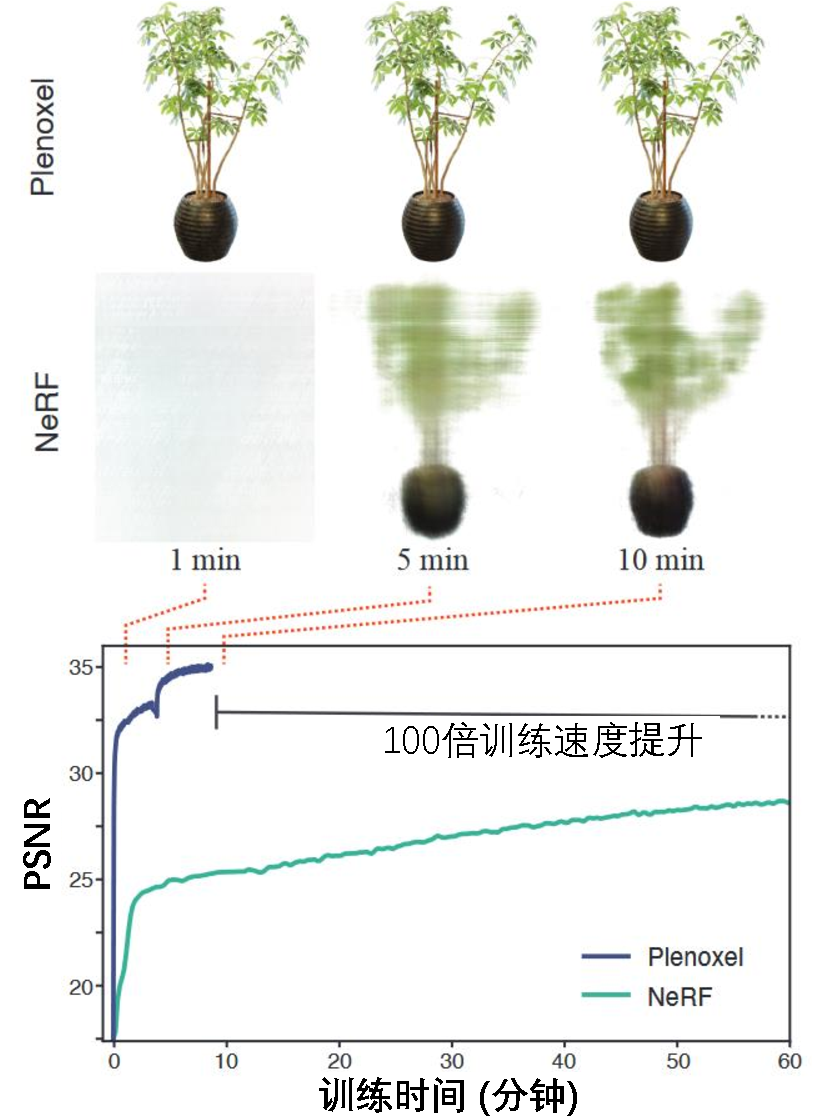
\includegraphics[width=.5\textwidth]{undergraduate-thesis/images/related-work/plenoxels-result.pdf}
    \caption{Plenoxels\cite{fridovich-keil_plenoxels_2022}和原始NeRF\cite{mildenhall_nerf_2020}的性能对比}
    \label{fig:related-work plenoxels-result}
\end{figure}

图\ref{fig:related-work plenoxels-result}中展示了Plenoxels方法和NeRF方法的性能对比,其中横轴为训练时间,纵轴为PSNR指标(越高越好)。由图可知,使用密集体素网格可以为隐式场训练带来成百倍的速度提升,且在最终渲染的效果上也要优于基于多层感知机的方法。

除此以外,当使用密集体素网格重建三维隐式表面时,由于体素网格不能提供多层感知机中的平滑特性(本文将在\ref{sec: related-work density-distance fields}节中讨论该特性),重建的三维表面通常会出现嘈杂的现象(图\ref{fig:related-work monosdf result})。

\subsubsection{隐式体素参数网格地图}
虽然上述的密集体素网格在渲染速度和效果上均有较大的提升,然而在面对更大规模的场景时,仅使用密集网格存储隐函数信息的网络表达能力并不足够,且使用密集网格进行表面重建也会遇到嘈杂的结果,为此,人们提出在网格中存储空间特征而非显式的隐函数值\cite{liu_neural_2021, takikawa_neural_2021, yu_monosdf_2022, huang_di-fusion_2021, peng_convolutional_2020},并使用一个后续的多层感知机解码器来计算最终隐函数值。

记分辨率为$R\times R\times R$的参数网格为$\Phi_\theta$, 多层感知机解码器为$f_\theta$,则使用参数网格来计算隐式函数值可以表示为:
\begin{equation}
    \hat{s} = f_\theta(\gamma(\mathbf{x}), \mathtt{interp}(\mathbf{x}, \Phi_\theta),
\end{equation}
其中$\gamma(\mathbf{x})$为$\mathbf{x}$的位置编码,本文将在\ref{sec: related-work positional encoding}一节讨论位置编码。

在此指上,为了进一步提高网络在场景细节上的建模能力,人们引入了多分辨率的体素参数网格地图\cite{yu_monosdf_2022},即使用多个不同分辨率的网格$\{\Phi^l_\theta\}^L_{l=1}$代替单一参数网格$\Phi_\theta$。记所有不同分辨率的网格中最小的网格($l=1$)的分辨率为$R_{\min}^3$,最大的网格($l=L$)分辨率为$R_{\max}^3$,则第$l$大的网格的分辨率可以表示为:
\begin{equation}
    R_l:=R_{\min}\cdot b^l, \quad l=\mathtt{floor}(\exp(\frac{1}{L - 1}(\ln R_{\max} - \ln R_{\min}))),
\end{equation}
进一步,查询多分辨体素参数网格的过程可以表示为:
\begin{equation}
    \hat{s} = f_\theta(\gamma(\mathbf{x}), \mathtt{concat}\{\mathtt{interp}(\mathbf{x}, \Phi_\theta^l)\}_{l=1}^L),
\end{equation}
$\mathtt{floor}$为下取整函数,$\mathtt{concat}$表示参数拼接。

\begin{figure}[ht]
    \centering
    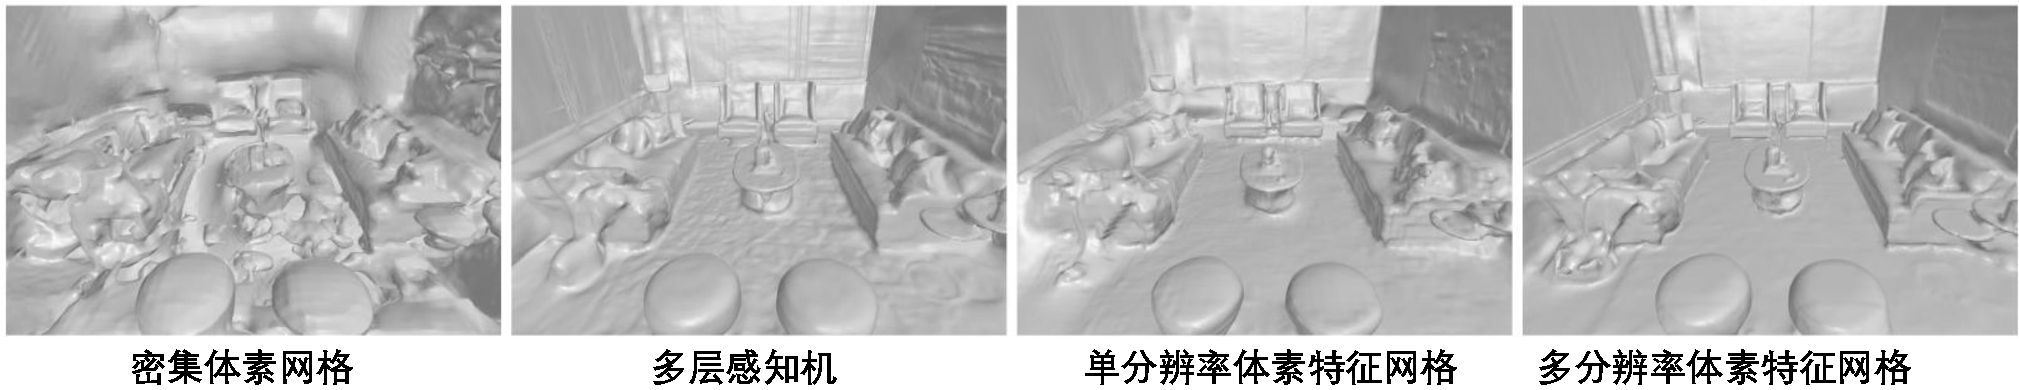
\includegraphics[width=\textwidth]{undergraduate-thesis/images/related-work/monosdf-result.pdf}
    \caption{使用多层感知机、密集体素网格、体素特征网格和多分辨率体素特征网格进行场景SDF学习的结果\cite{yu_monosdf_2022}。}
    \label{fig:related-work monosdf result}
\end{figure}

本文在图\ref{fig:related-work monosdf result}中比较神经隐式表面表示的不同设计选择,观察到密集的 SDF 网格会导致嘈杂的重建结果,而 MLP 和单分辨率体素网格改进了结果,但重建的几何图形往往过于平滑而缺少细节,使用多分辨率体素网格可获得较好的结果。

\subsubsection{基于哈希编码的体素参数网格地图}
由于体素参数地图方法在存储大规模场景时,需要使用高分辨率的参数网格来获得足够的细节并保证精度,这导致了空间复杂度高达$\mathcal{O}(N^3)$。然而,在三维场景中,人们通常只关注表面,其所需要的数据量只随场景大小呈平方的空间复杂度($\mathcal{O}(N^2)$)。为了解决这一问题,M\"uller等人提出了一种基于哈希编码的体素参数网格地图——InstantNGP\cite{muller_instant_2022}。 InstantNGP使用哈希表来存储隐式函数值,只需控制哈希表的大小随场景大小平方增长即可。

\begin{figure}[ht]
    \centering
    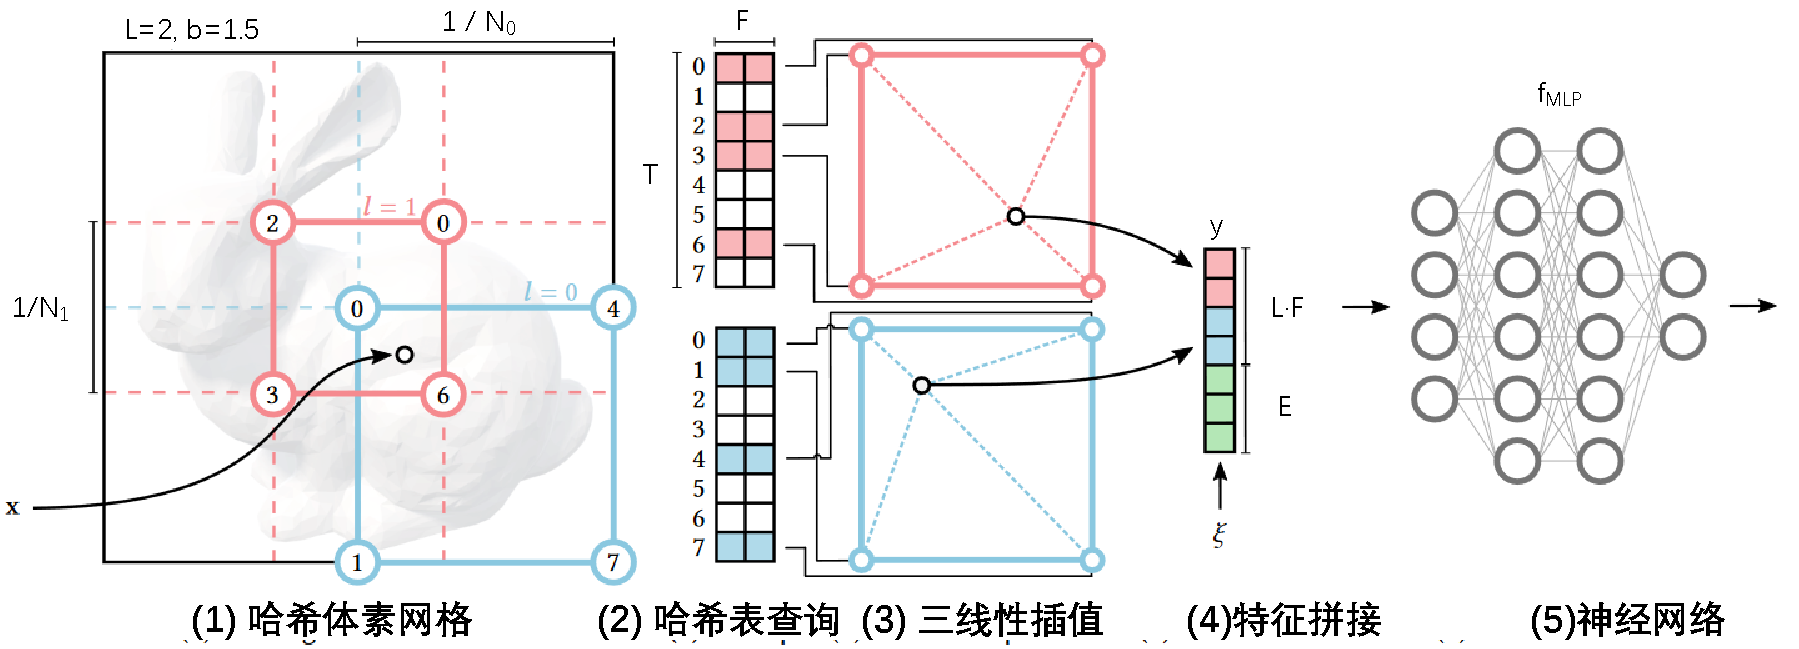
\includegraphics[width=\textwidth]{undergraduate-thesis/images/related-work/instantngp.pdf}
    \caption{InstantNGP\cite{muller_instant_2022} 方法流程图}
    \label{fig:related-work instantngp}
\end{figure}

如图\ref{fig:related-work instantngp}所示,InstantNGP沿用了多分辨率体素网格的基本框架,在查询任意一点的三维场景隐函数值时,首先需要查询其在各个层次的网格上的八个相邻节点,接着将节点编号作为索引查询哈希表,将查询结果经三线性插值之后拼接形成三维点特征。可以将这个过程表示为:
\begin{equation}
    \hat{s} = f_\theta(\gamma(\mathbf{x}), \mathtt{concat}\{\mathtt{interp}(h^l(\mathbf{x}), \Phi_\theta)\}_{l=1}^L),
\end{equation}
其中$h^l(\mathbf{x})$为哈希函数,在InstantNGP中,每个级别的参数网格使用不同的哈希函数:
\begin{equation}
    h^l(\mathbf{x}) = \left(\bigoplus_{i}x_i\pi_i^l\right) \text{mod} T,
\end{equation}
$T, \pi^l$为随机大质数。

\subsubsection{基于张量分解的向量-矩阵地图表示}
虽然InstantNGP基于哈希表的存储数据结构可以有效地缓解基于体素网格的场景表示中高空间复杂性的问题,然而研究者发现现有方法所使用的体素网格中绝大部分体素均属于空白空间,因而网格的使用率实际并不高。Anpei等人\cite{chen_tensorf_2022}的工作TensoRF中利用了一个事实,即特征网格可以自然地被视为 4D 张量,其中它的三个模式对应于网格的 XYZ 轴,第四个模式代表特征通道维度,从而解决了体素网格表示的低效问题,从而产生了一系列简单而有效的方法。TensoRF利用经典张量分解技术(已广泛应用于各个领域的高维数据分析和压缩 \cite{kolda_tensor_2009}),将辐射场的张量分解为多个低秩张量分量,从而获得准确且紧凑的场景表示。

\begin{figure}[ht]
    \centering
    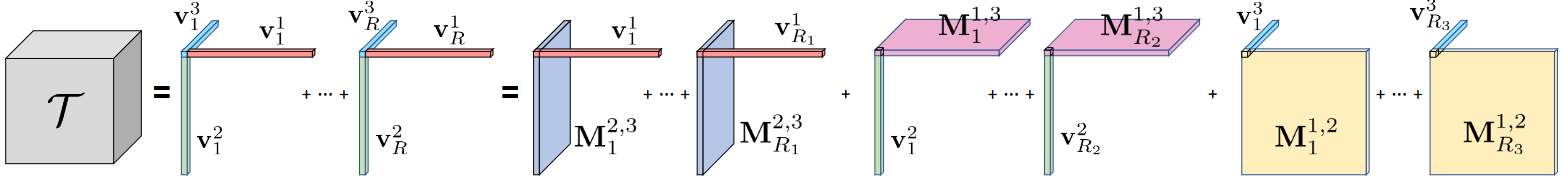
\includegraphics[width=\textwidth]{undergraduate-thesis/images/related-work/Tensor Decomp.png}
    \caption{张量分解\cite{chen_tensorf_2022}。左图:CP 分解,它将张量分解为向量外积之和。右图:TensoRF的向量矩阵分解,它将张量分解为向量矩阵外积的总和。}
    \label{fig:related-work tensor-decomp}
\end{figure}

传统的CP张量分解(如式\ref{eq: related-work CP decomp}所示),将三维张量$\mathcal{T}\in\mathbb{R}^{I\times J\times K}$分解为三组秩为一的向量乘积的和。TensoRF将CP分解拓展为向量-矩阵分解模式(如式\ref{eq: related-work TensoRF decomp}所示)。对于每个分解单元,将CP-分解中的其中两个分量合并,不使用单独的向量,而是组合每两个模式并用矩阵表示它们,从而允许每个分解单元使用较少数量的组件进行充分参数化。
\begin{equation}
    \mathcal{T} = \sum_{r=1}^R\mathbf{v}_r^1\circ\mathbf{v}_r^2\circ\mathbf{v}_r^3
    \label{eq: related-work CP decomp}
\end{equation}

\begin{equation}
    \mathcal{T} = \sum_{r=1}^R\mathbf{v}_r^X\circ\mathbf{M}_r^{Y,Z}+\mathbf{v}_r^Y\circ\mathbf{M}_r^{X,Z}+\mathbf{v}_r^Z\circ\mathbf{M}_r^{X,Y}
    \label{eq: related-work TensoRF decomp}
\end{equation}

TensorRF (VM)使用一组向量 ($\mathbf{v}$) 和矩阵 ($\mathbf{M}$) 将辐射场建模为张量,它们沿相应的 (XYZ) 轴描述场景,并用于计算可微分光线行进中的体积密度 $\sigma$ 和视角相关颜色 $c$。对于每个着色位置$ \mathbf{x} = (x, y, z)$,使用来自向量/矩阵因子的线性/双线性插值结果来有效地计算张量分量的特征。该特征被进一步用于渲染,从而得到一个紧致的神经隐式表示。

\begin{figure}[ht]
    \centering
    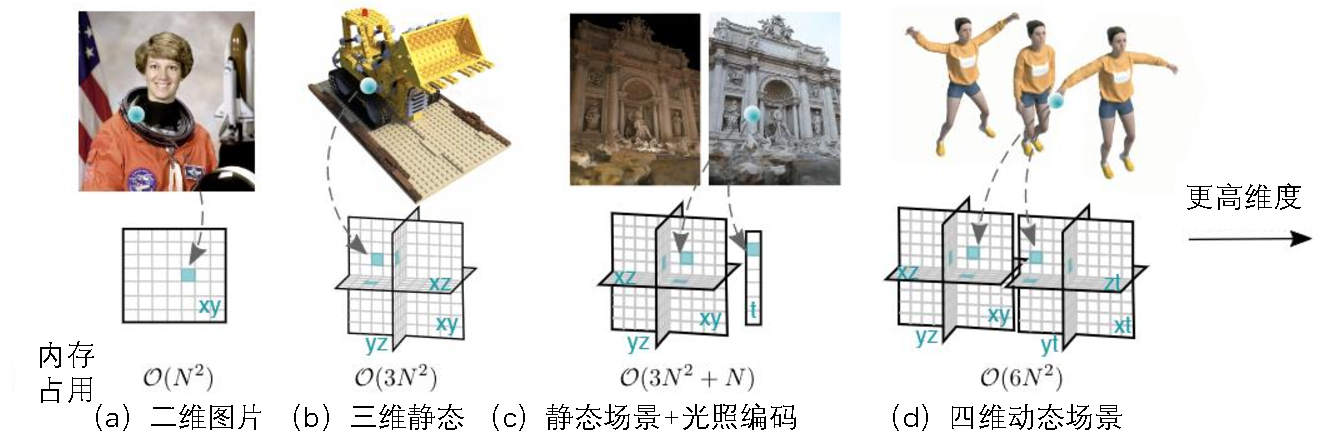
\includegraphics[width=\textwidth]{undergraduate-thesis/images/related-work/kplanes-teaser.pdf}
    \caption{$d$ 维空间的平面分解示意图\cite{fridovich-keil_k-planes_2023}。}
    \label{fig:related-work kplane-teaser}
\end{figure}

\subsubsection{多平面地图表示}
受TensoRF启发,研究者进一步将张量分解的概念进一步泛化,仅使用多个互相正交的平面来代替体素网格\cite{fridovich-keil_k-planes_2023, cao_hexplane_2023, reiser_merf_2023, chan_efficient_2022}。其中K-Planes\cite{fridovich-keil_k-planes_2023}将$d$维体素张量使用$k=\frac{d(d-1)}{2}$个平面表示,即$d$个维度的任意两维均用一个平面表示,如图\ref{fig:related-work kplane-teaser}所示。例如,对于静态 3D 场景,这会产生三平面,其中3个平面代表 XY、XZ 和 YZ。而对于动态 4D 场景,这会产生六平面,其中6 个平面,包括三个纯空间平面和三个时空平面 X-t、Y-t 和 Z-t。如果希望表示一个 5D 空间,可以使用$\frac{5\times4}{2}=10$个平面。


\begin{figure}[ht]
    \centering
    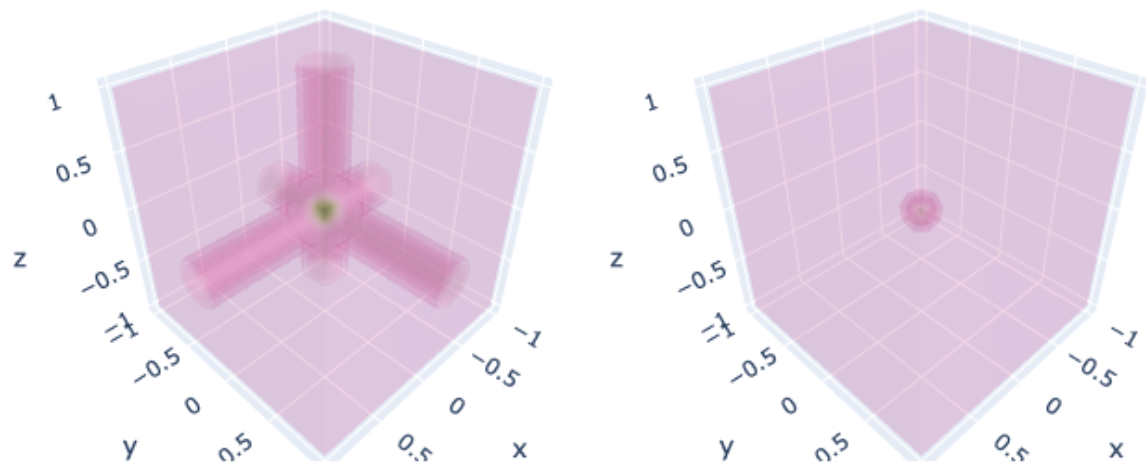
\includegraphics[width=\textwidth]{undergraduate-thesis/images/related-work/hadamard-product.png}
    \caption{平面特征的逐元素加法(左)与乘法(右)的比较。在这两种情况下,假设每个平面中只有单个条目为+1,其余部分均为零,通过乘法可以选择单个 3D 点,但通过加法只能产生相交线。这说明乘法可以提高显式模型的表达能力\cite{fridovich-keil_k-planes_2023}。}
    \label{fig:related-work hadamard-product}
\end{figure}

不同于最早的三平面场景表示\cite{chan_efficient_2022}中使用逐像素的求和来整合各平面上的特征,K-Planes中使用Hadamard乘积来获取空域感知的特征信号(如\ref{fig:related-work hadamard-product}所示),即:
\begin{equation}
    f(\mathbf{q}) = \prod_{c\in C}f(\mathbf{q})_c,
\end{equation}
其中$c\in C$为场景中的平面集合,在每个平面中查询$\mathbf{q}$点处的特征,通过逐像素求乘积得到高维空间中点的特征。

\noindent\textbf{小结:}
本节介绍了神经隐式场出现以来,所使用的场景表示从多层感知机\cite{mildenhall_nerf_2020,park_deepsdf_2019, mescheder_occupancy_2019, shim_snerl_2023, zhi_-place_2021}逐渐发展为体素网格\cite{fridovich-keil_plenoxels_2022,yu_monosdf_2022,muller_instant_2022,jiang_instantavatar_2022}、多平面\cite{chen_tensorf_2022,fridovich-keil_k-planes_2023,cao_hexplane_2023}等场景表示方法。
虽然多平面的方法可以对一个简单场景进行高效、准确的表示学习,但当场景规模逐渐从物体、室内场景基本扩展到室外自动驾驶大场景下时,使用单一的多平面场景表示反而会产生退化的效果。本文将提出一种混合场景表示方法,使得即便在更大规模的复杂场景中,依然可以用较小的存储空间获得准确的场景表示。


\section{真实感的神经渲染方法:场景扭曲变换}
\label{sec: related-work realistic rendering}
除了使用不同的场景表示方法外,为了实现更真实的渲染效果,研究者还在其他方面做出了改进。其中,最为典型的方法是将三维欧式空间通过变换,映射到扭曲后的参数空间。

通常来讲,在场景图片数据集中,场景的内容在三维空间上并不是均匀分布的,如在前向观察的数据集中,通常场景内容随着深度的增加而反比例下降;在无边界、物体中心的数据集中,场景内容随着空间点到物体中心距离的增加而下降。因此,若能将在原始三维欧式空间中非均匀分布的空间点映射到一个均匀分布,则将能大大提升场景表示的利用率,从而提高渲染真实感。

\subsection{位置编码}
\label{sec: related-work positional encoding}

尽管神经网络被证明为通用的函数逼近器\cite{hornik_multilayer_1989},但研究者发现让网络直接在 输入坐标$(x,y,z,\theta,\phi)$上优化会导致渲染颜色。机器学习领域相关工作\cite{rahaman_spectral_2019}表明多层感知机偏向于学习低频函数,在高频信息上的学习速率显著低于低频信息的学习速率。而在将输入传递到网络之前,使用高频函数将输入映射到更高维空间可以更好地拟合包含高频变化的数据。

位置编码是一种常用于自注意力机制的技术,它通过将空间位置信息编码为向量来提高神经网络的表现力。但是Transformers\cite{vaswani_attention_2017}等基于注意力机制的方法为Token在整个序列中的离散位置提供隐式的位置坐标,然而在NeRF\cite{mildenhall_nerf_2020}中,通过将场景中的位置信息编码为含有位置信息的高维向量,可以将输入的xyz坐标映射到高维空间中,从而让网络学习场景中的高频细节信息,实现更真实的渲染效果。NeRF位置编码将输入数据$p$通过式\ref{eq: related-work PE}所示的方法映射到高维频域空间。
\begin{equation}
    \gamma(p) = \left(\sin(2^0\pi p),\cos(2^0\pi p),\cdots \sin(2^{L-1}\pi p),\cos(2^{L-1}\pi p)\right)
    \label{eq: related-work PE}
\end{equation}

\begin{figure}[ht]
    \centering
    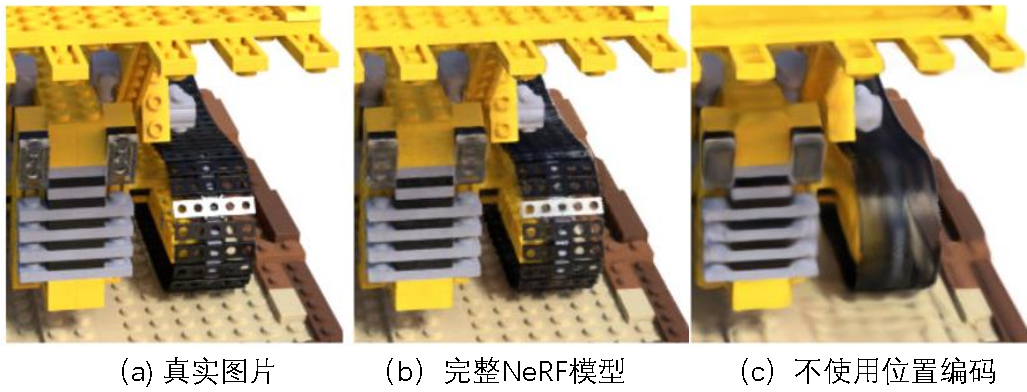
\includegraphics[width=\textwidth]{undergraduate-thesis/images/related-work/NeRF ablation-PE.pdf}
    \caption{位置编码对NeRF网络性能的影响\cite{mildenhall_nerf_2020}。}
    \label{fig:related-work nerf-PE-ablation}
\end{figure}

图\ref{fig:related-work nerf-PE-ablation}中展示了去掉位置编码后对NeRF网络渲染图片的效果影响。由图可以看出,去除高频位置信息后,NeRF网络很难表示图片中的高维几何细节,从而表现出“模糊”的特点。

从本质上,NeRF的位置编码实质上也是一个扭曲变换,将信息分布不均匀的空域映射到更加均匀的频域空间。

\subsection{基于Mip的反走样神经渲染}
尽管神经辐射场\cite{mildenhall_nerf_2020}及其变体\cite{muller_instant_2022,martin-brualla_nerf_2021,zhang_nerf_2020}在视图合成任务中展示了令人印象深刻的结果,但 NeRF 的渲染模型存在缺陷:当训练图像以多种分辨率观察场景内容,或分别从远处和近处观察同一位置时,NeRF的渲染在近景视图中显得过于模糊,并且在远景视图中包含混叠伪影。其原因在于NeRF将一个像素抽象为一个无穷小的没有面积的三维点,然而在真实世界中,像素在空间上占有一定的面积,从而相机发出的“光线”实际上应该表示为一个圆锥体(如图\ref{fig:related-work mip-nerf cone tracing}所示)。式\ref{eq: related-work volume rendering}中的NeRF渲染公式仅在一条射线上积分所有的辐射值,使用线积分的结果代替了视锥中全部三维点的重积分:
\begin{equation}
    c = \iiint_{\mathbf{p}\in V}\sigma(\mathbf{p})T(\mathbf{p})c(\mathbf{p},\mathbf{d})\text{d}p,
\end{equation}
其中$V$为相机原点$\mathbf{o}$朝方向$\mathbf{d}$发射的视锥,$p$为$V$中点。

\begin{figure}[ht]
    \centering
    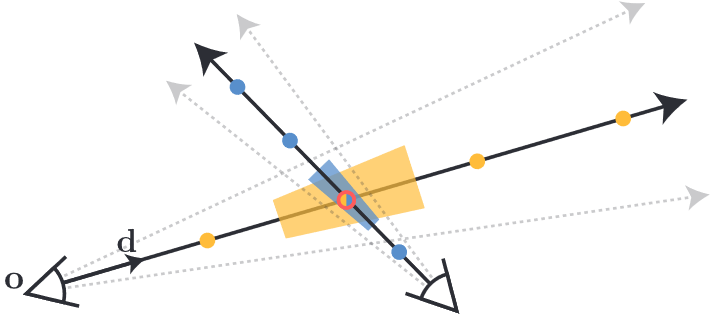
\includegraphics[width=0.8\textwidth]{undergraduate-thesis/images/related-work/mipnerf-intersection.png}
    \caption{NeRF方法产生走样原因的示意图\cite{barron_mip-nerf_2021}。}
    \label{fig:related-work mip-nerf intersection}
\end{figure}

这样的简化必然会导致渲染误差的存在,进而产生走样的渲染结果。如图\ref{fig:related-work mip-nerf intersection}所示,当分别从两个不同远近、不同角度的视角同时观察到空间中的某个三维点。NeRF沿着每个像素的光线提取点采样位置编码特征,这些点采样特征忽略了每条射线观察到的体积的形状和大小,因此两个不同的相机以不同的比例对同一位置进行成像可能会产生相同的模糊点采样特征,从而显着降低 NeRF 的性能。

\begin{figure}[ht]
    \centering
    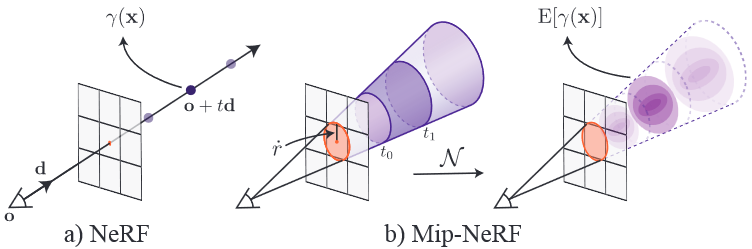
\includegraphics[width=\textwidth]{undergraduate-thesis/images/related-work/mipnerf-cone.png}
    \caption{NeRF (a) 沿着从相机投影中心通过每个像素的光线进行采样,然后使用位置编码 (PE) $\gamma$ 对这些点进行编码以产生特征$\gamma(x)$。 Mip-NeRF (b) 对由相机像素定义的 3D 圆锥台进行推理,使用集成位置编码 (IPE) 对这些锥形截锥体进行特征化,使用多元高斯近似截锥体,然后计算积分 $E[\gamma(x)]$以近似超采样的效果\cite{barron_mip-nerf_2021}。}
    \label{fig:related-work mip-nerf cone tracing}
\end{figure}

一个直接的解决方案是采用离线光线追踪中使用的策略:通过发射多条光线并对每个像素进行超采样。但这对于像 NeRF 这样的神经体积表示来说是非常昂贵的,它需要数百次查询多层感知机网络来渲染一条射线,并需要几个小时甚至几天来重建一个场景。Mip-NeRF \cite{barron_mip-nerf_2021}提出将采样过程显式建模为投射锥体而不是射线的过程,并对每个采样的锥台使用一个各向异性的高斯椭球表示。

为了模拟对整个锥台进行超采样,Mip-NeRF提出用高斯椭球上位置编码的均值近似每个锥台内体积的位置编码的平均,即集成位置编码(Integrated Positional Encoding,IPE)。
\begin{figure}[ht]
    \centering
    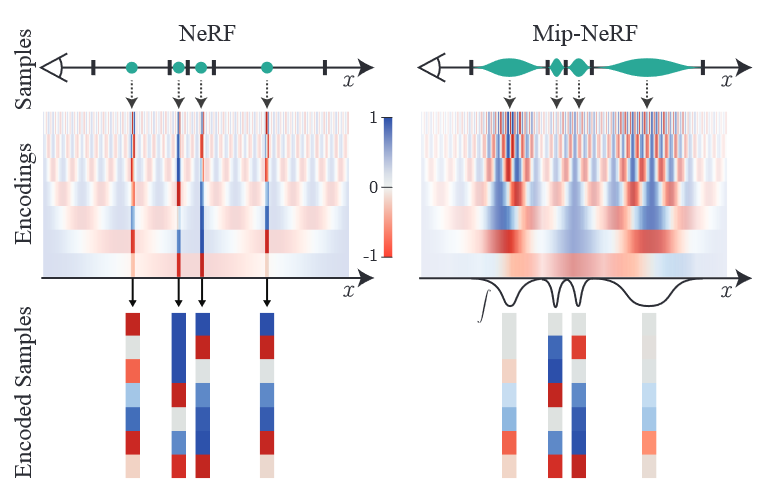
\includegraphics[width=\textwidth]{undergraduate-thesis/images/related-work/mipnerf-encoding.png}
    \caption{NeRF(左)和集成位置编码(IPE)(右)的一维可视化。由于 NeRF 沿每条射线对点进行采样并对所有频率进行同等编码,因此高频 PE 特征混叠,从而导致渲染伪影。通过在每个区间上使用集成位置编码特征,当频率周期与被集成的间隔大小相近时,IPE特征的高频维度缩小到零,从而产生隐式编码大小的抗锯齿特征。\cite{barron_mip-nerf_2021}}
    \label{fig:related-work mip-nerf encoding}
\end{figure}

具体来讲,高斯椭球$(\mu,\Sigma)$内的集成位置编码可以写作:
\begin{align}
    \gamma(\mu,\Sigma) &= \text{E}_{\mathbf{x}\sim\mathcal{N}(\mu_\gamma,\Sigma_\gamma)}[\gamma(\mathbf{x})] \\
    &= \begin{bmatrix}
    \sin(\mu_\gamma)\circ\exp(-\frac{1}{2}\text{diag}(\Sigma_\gamma))\\
    \cos(\mu_\gamma)\circ\exp(-\frac{1}{2}\text{diag}(\Sigma_\gamma))
    \end{bmatrix}
\end{align}

由图\ref{fig:related-work mip-nerf encoding},IPE 特征的行为很直观:如果位置编码中的特定频率的周期大于用于构造 IPE 特征的区间宽度,则该频率的编码不受影响。但是,如果周期小于间隔,则该频率的编码将按比例缩小至零。简而言之,IPE 保留了在一个区间内恒定的频率并温和地“移除”在一个区间内变化的频率,而 PE 保留了直到某个手动调整的超参数 L的所有频率。通过以这种方式缩放每个三角函数值,IPE可以有效地抗锯齿位置编码功能,可以平滑地编码空间体积的大小和形状。

\begin{figure}[ht]
    \centering
    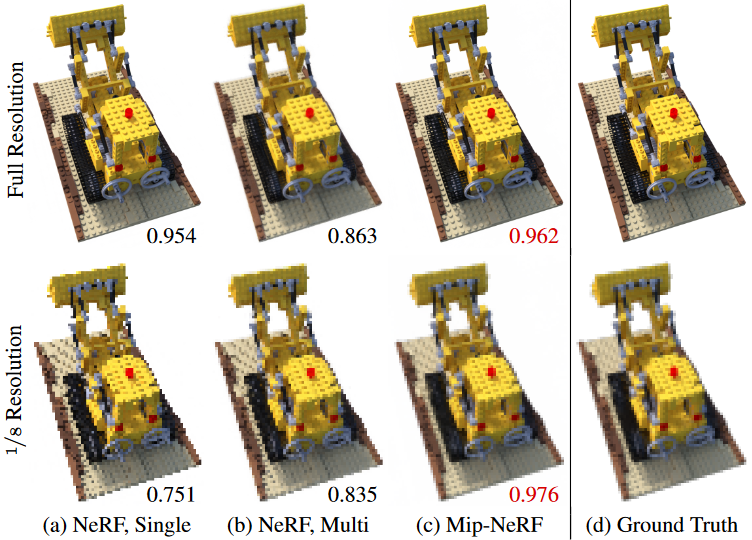
\includegraphics[width=0.8\textwidth]{undergraduate-thesis/images/related-work/mipnerf-multi-scale.png}
    \caption{Mip-NeRF\cite{barron_mip-nerf_2021} 和基线模型在不同图片分辨率上渲染的效果对比。}
    \label{fig:related-work mip-nerf results}
\end{figure}

图\ref{fig:related-work mip-nerf results}展示了Mip-NeRF使用IPE后与其他模型在渲染低分辨率图像时的效果对比。在全分辨率图像上训练的 NeRF 能够在新的视图位置生成逼真的渲染图,但仅限于训练图像的分辨率或比例;将相机向后拉并放大(或类似地,调整相机内在特性以降低图像分辨率)会导致呈现出严重的锯齿现象;在多分辨率图像上训练 NeRF 可以稍微改善这个问题,但会导致跨尺度渲染质量差:全分辨率模糊,低分辨率出现“锯齿”; Mip-NeRF也在多分辨率图像上训练,但能够在不同尺度上生成逼真的渲染。

\subsection{无界场景表示}
相比原始的位置编码和Mip-NeRF中的集成位置编码,Mip-NeRF中的无界场景映射则是一种更加直观的扭曲映射方法。

由于透视投影,远离相机放置的物体将占据图像平面的一小部分,但如果放置在附近,则会占据更多图像并且细节可见。因此,理想的 3D 场景参数化应该为附近的内容分配更多的容量,为远处的内容分配更少的容量。

最初的 NeRF 论文侧重于从360$^\circ$捕获具有蒙版背景的对象以及所有图像面向大致相同方向的正面场景(也称作Forward-Facing)。对于蒙面物体,NeRF 直接参数化 3D 欧几里得空间中的场景,但对于正面场景,NeRF 使用投影空间中定义的坐标(归一化设备坐标,或“NDC”空间)。通过将无限深的相机视锥变形为有界立方体,其中沿 z 轴的距离对应于视差(反距离),NDC 以与透视投影的几何形状一致的方式有效地重新分配 NeRF MLP 的容量。然而,在所有方向上都是无界的场景,而不仅仅是在一个方向上,需要不同的参数化。 不同于NeRF++\cite{zhang_nerf_2020}使用额外的网络对远处的物体进行建模,在Mip-NeRF 360\cite{barron_mip-nerf_2022}中,将这个想法扩展到 Mip-NeRF 并提出了一种将任何平滑参数化应用于体积的无界场景参数化方法。

\begin{figure}[ht]
    \centering
    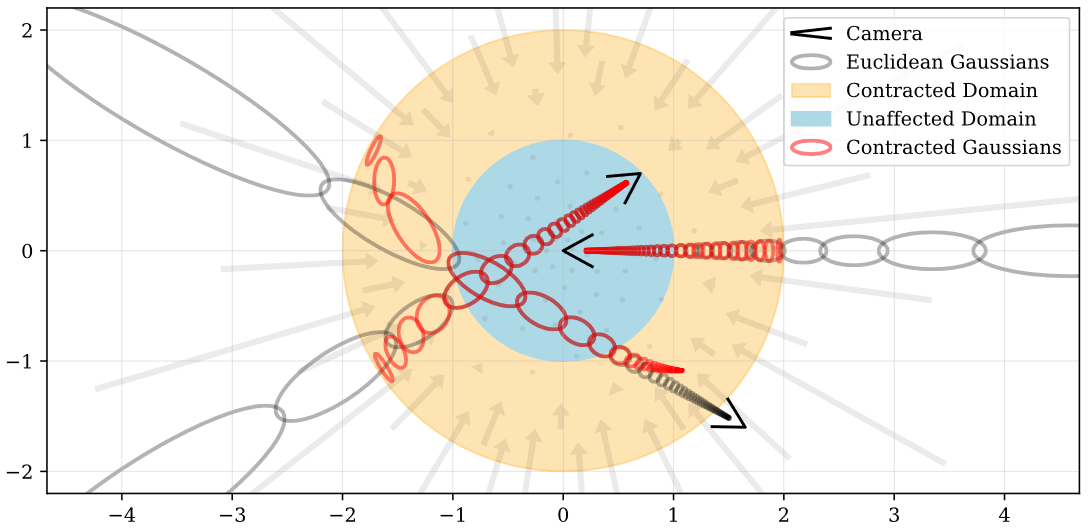
\includegraphics[width=\textwidth]{undergraduate-thesis/images/related-work/mipnerf360-contraction.png}
    \caption{Mip-NeRF 360\cite{barron_mip-nerf_2022}的无界场景压缩的二维示意图}
    \label{fig:related-work-unbounded-contraction}
\end{figure}

如图\ref{fig:related-work-unbounded-contraction}所示,对于任意一个输入坐标$x\in\mathbb{R}^3$,Mip-NeRF 360将输入坐标通过下面的公式映射到一个半径为2的球面内:
\begin{equation}
    \mathtt{contract}(\mathbf{x}) = \left\{\begin{matrix}&\mathbf{x}&||\mathbf{x}||<1\\&(2-\frac{1}{||\mathbf{x}||})(\frac{\mathbf{x}}{||\mathbf{x}||})&||\mathbf{x}||\geq1\end{matrix}\right.
\end{equation}

\noindent\textbf{小结:}
本节介绍了使用场景扭曲变换提高场景表示模型利用率的几种方法,然而目前的扭曲变换方法无法解决在更大规模的室内、室外复杂场景的高效表达,因而限制了神经隐式场在自动驾驶等领域的发展。本文提出基于神经点云的场景扭曲变换,使得场景表示可以自适应地拟合大规模场景。



\section{辐射-距离混合隐式场}
\label{sec: related-work density-distance fields}
本章的前两节介绍了以神经辐射场的神经场景表示的发展,然而单一的辐射场景表示对于场景几何的建模能力较差。本节将首先分析辐射场这一不足的原因,接着分别从采样策略、体渲染模型、多元传感信息融合和混合隐式场优化的几个方面介绍辐射-距离混合隐式场。

\subsection{采样策略}
神经辐射场中首次将隐式表达用于体积渲染积分的管线中,然而在计算机实现中必须对体积积分进行离散化,使用有限的采样点最大限度地还原连续体积中的密度分布。因此,选取合适数量、位置的采样点对于隐式场场景表示学习格外重要。本节首先介绍NeRF\cite{mildenhall_nerf_2020}中的分层采样方法,接着介绍后续工作中对该方法的改进。

\subsubsection{分层采样}
\label{sec: coarse-to-fine sampling}
在原始NeRF中,为了估计体渲染积分(公式\ref{eq: related-work volume rendering}),使用了由粗到精的分层采样策略:首先将$[t_n,t_f]$划分为N个均匀分布的区间,然后从每个区间内随机均匀地抽取一个样本(如式\ref{eq: related-work coarse-sampling}),将这些样本通过粗网络后根据体密度分布进行重要性重采样得到精细样本,最后将两次抽取的采样点通过精细网络进行渲染。
\begin{equation}
    t_i\sim\mathcal{U}\left[t_n+\frac{i-1}{N}(t_f-t_n), t_n+\frac{i}{N}(t_f-t_n)\right]
    \label{eq: related-work coarse-sampling}
\end{equation}

在NeuS\cite{wang_neus_2021}中,进一步改良了这种基于重要性的分层采样,使用同一网络进行多次的分层抽取采样点,来实现在表面出更多采样,而在自由空间中减少采样的目的。


\subsubsection{隐式表面引导的采样}
在混合隐式表达中,由于隐式表面模型建模了三维点到表面的距离信息,而隐式表面模型的关键假设是只有与表面的第一个交点处的区域对渲染方程有贡献。可以较为方便地通过射线传播模型求解表面坐标$\mathbf{x}_s$\cite{niemeyer_differentiable_2020}。

UNISURF\cite{oechsle_unisurf_2021}在早期迭代期间,会使用类似NeRF中的粗采样策略在整个体积空间中随机采样。在后期的迭代中,样本点采样会更靠近估计的表面。由于可以通过求根法\cite{niemeyer_differentiable_2020}直接从占用场估计表面,因此无需像 NeRF 中那样进行分层两阶段采样。

\begin{figure}[ht]
    \centering
    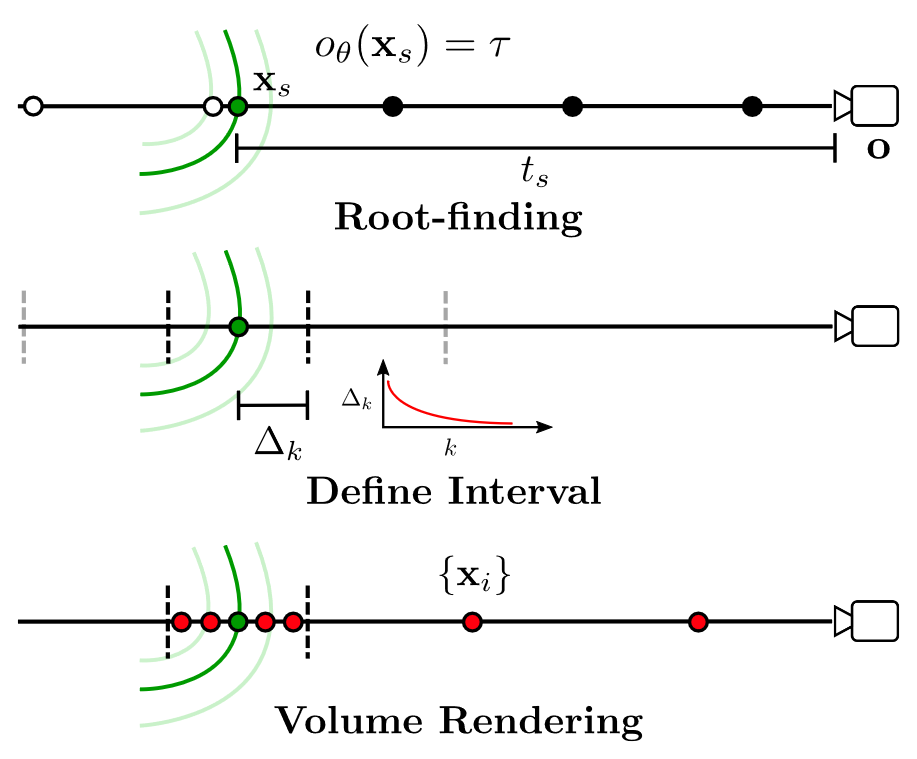
\includegraphics[width=0.8\textwidth]{undergraduate-thesis/images/related-work/unisurf-sampling.png}
    \caption{UNISURF\cite{oechsle_unisurf_2021}采样策略示意图}
    \label{fig:related-work unisurf-sampling}
\end{figure}

\subsubsection{基于误差的采样}
VolSDF\cite{yariv_volume_2021}中给出了使用符号距离场估计的不透明度$\hat{O}$的估计误差的上界:
\begin{equation}
    |O(t)-\hat{O}(t)|\leq B_{\mathcal{T},\beta}
\end{equation}

其中$B_{\mathcal{T},\beta}<\varepsilon$存在两种可能性:
\begin{enumerate}
    \item 当超参数$\beta$固定时,对于任意给定$\varepsilon$,总存在一个足够稠密的采样点集$\mathcal{T}$使得$B_{\mathcal{T},\beta}<\varepsilon$
    \item 当采样点数目$n$固定时,对于任意给定$\varepsilon$,总存在一个足够大的$\beta$使得$B_{\mathcal{T},\beta}<\varepsilon$:
    \begin{equation}
        \beta\geq\frac{\alpha t_f^2}{4(n-1)\log(1+\varepsilon)}.
        \label{eq: related-work volsdf beta-error}
    \end{equation}
\end{enumerate}

基于这一观察,VolSDF设计了一个基于误差的重采样方法:首先使用均匀采样获得初始采样点集$\mathcal{T}=\mathcal{T}_0$,通过公式\ref{eq: related-work volsdf beta-error}计算出所需要的$\beta_+$使得误差在要求范围内,接着迭代地对采样点集进行上采样,并逐步减少$\beta$直至收敛。

\begin{figure}[ht]
    \centering
    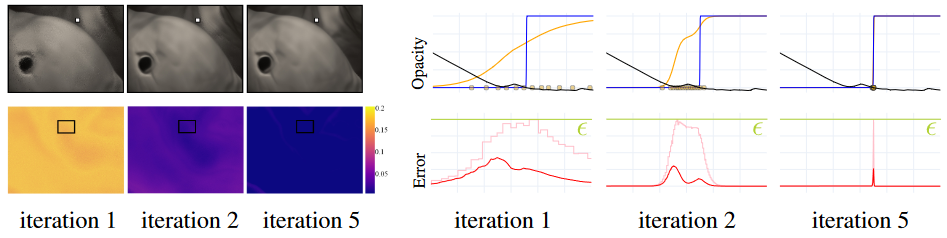
\includegraphics[width=\textwidth]{undergraduate-thesis/images/related-work/volsdf-sampling.png}
    \caption{VolSDF\cite{yariv_volume_2021}基于误差的重采样过程。}
    \label{fig:related-work volsdf-sampling}
\end{figure}

图\ref{fig:related-work volsdf-sampling}展示了VolSDF采样的迭代过程,经过数次上采样后,网络可以以很少的采样点对不透明度进行准确的估计,使得误差在要求范围内。VolSDF得到的场景几何如图\ref{fig:related-work volsdf-result}所示,由图可见VolSDF可以产生比NeRF更加准确的场景几何。

\begin{figure}[ht]
    \centering
    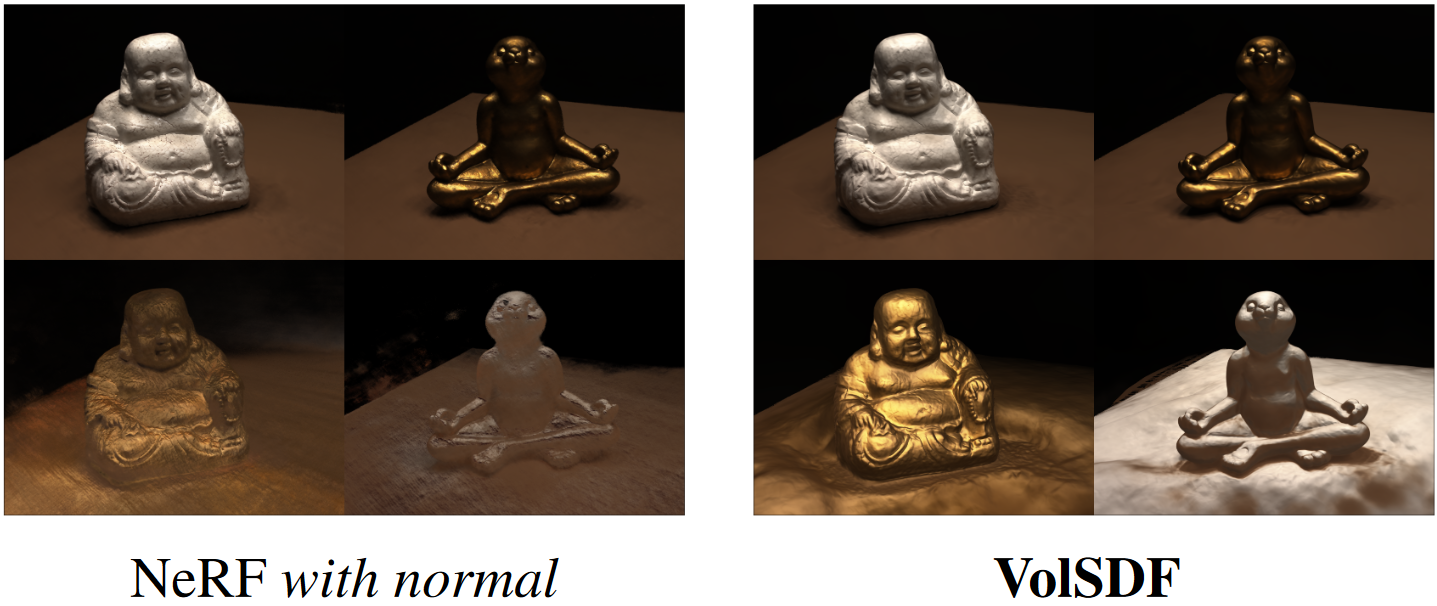
\includegraphics[width=0.7\textwidth]{undergraduate-thesis/images/related-work/volsdf-result.png}
    \caption{VolSDF\cite{yariv_volume_2021}的场景几何。}
    \label{fig:related-work volsdf-result}
\end{figure}

% \subsubsection{基于Proposal网络的采样}


\subsubsection{基于Occupancy的网格采样}
为了提升采样效率,InstantNGP\cite{muller_instant_2022}提出使用基于占用网格的采样:当沿着光线行进进行训练和渲染时,InstantNGP希望放置样本,使它们对图像的贡献尽量均匀,从而最大限度地减少计算浪费。因此,他们通过维护一个粗略标记空与非空空间的占用网格来集中表面附近的样本。

\subsection{体渲染方法}
混合隐式场景表示中,为了同时优化符号距离场和神经辐射场,通常需要将符号距离转换成体密度来进行体积渲染,然而这一映射过程并不唯一,在这一部分中,这里介绍两种比较常见的映射。

\subsubsection{以VolSDF为代表的体渲染方法}
在体积渲染过程中,体密度$\sigma(\mathbf{x})$是一个$\mathbb{R}^3\to\mathbb{R}_+$的隐式标量函数,其值表达了光在$\mathbf{x}$点被阻挡的概率密度,也表示了该点处物体粒子的密集程度。在VolSDF\cite{yariv_volume_2021}中,作者通过一个闭式函数将符号距离值映射为体密度:
\begin{equation}
    \sigma(\mathbf{x}) = \alpha\Psi_\beta(-d_\Omega(\mathbf{x})),
    \label{eq: related-work volsdf equation}
\end{equation}
其中$\alpha,\beta$为超参数。

直观地说,体密度$\sigma$ 模拟了一个具有恒定密度$\alpha$的均匀物体,它在物体边界附近平滑减小,其中平滑程度由$\beta$控制。在式\ref{eq: related-work volsdf equation}中定义密度的好处有两方面:首先,它为表面几何形状$\mathcal{M}$提供了有用的归纳偏置,并提供了重建表面的原则性方法,即作为$\text{d}\Omega$的零值面。其次,式中定义的密度的特定形式有助于限制渲染体积的不透明度(或等效的透明度)误差,这是体积渲染管线中的一个重要组成部分。前面的章节探讨了$\beta$的大小对于重建误差$\varepsilon$的控制作用。

\subsubsection{以NeuS为代表的体渲染方法}
然而,VolSDF所提出的经验性公式没有考虑到光线上点的先后关系,经过转换的体密度值在计算权重时也会出现偏差。NeuS\cite{wang_neus_2021}方法基于这样的观察,提出任何的转换函数$g$应满足的两个条件:
\begin{enumerate}
    \item \textbf{无偏性}:对于任意给定射线$\mathbf{r}(t)$,经由转换映射计算出的体密度通过体积渲染得到的点权重$w(t)$应在物体表面处的权重取得极大值,即在表面$t^*$($f_\text{SDF}(t^*)$)处有$\sigma'(t) = 0$;
    \item \textbf{遮挡感知}:当空间中两点$P_i$,$P_j$分别对应深度$t_i$,$t_j$满足$f_{SDF} (P_i )=f_{SDF} (P_j ),t_i<t_j$,则在渲染时须有权重$w_i>w_j$。
\end{enumerate}

\begin{figure}[ht]
    \centering
    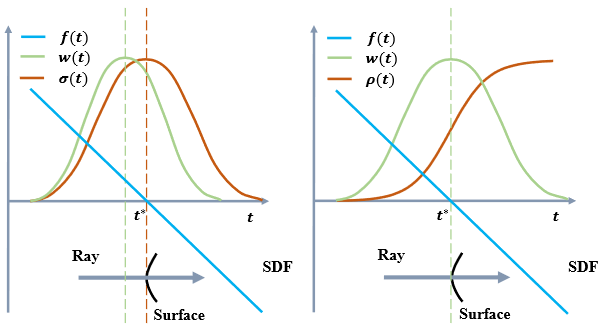
\includegraphics[width=0.9\textwidth]{undergraduate-thesis/images/related-work/neus conditions.png}
    \caption{NeuS\cite{wang_neus_2021}中提出的SDF到体密度映射函数的两个必要条件。左图所展示的传统解决方案并不能满足无偏性和遮挡感知的条件。}
    \label{fig: related-work neus conditions}
\end{figure}

如图\ref{fig: related-work neus conditions}所示,传统方法不能满足无偏和遮挡感知,因而NeuS提出了如下的转换方案:
\begin{equation}
    \sigma(t) = \max\left(\frac{-\frac{\text{d}\Phi_s}{\text{d}t}(f_{SDF}(t)}{\Phi_s(f_{SDF}(t))}, 0\right),
    \label{eq: related-work neus function}
\end{equation}
其中$\Phi_s$为Sigmoid函数的一阶导函数。

\begin{figure}[ht]
    \centering
    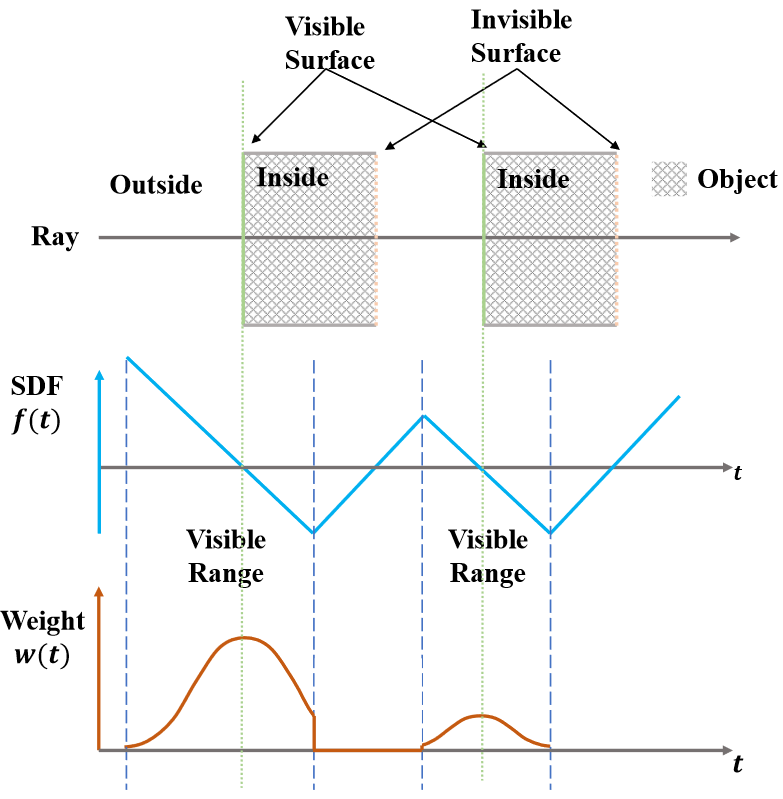
\includegraphics[width=0.8\textwidth]{undergraduate-thesis/images/related-work/neus multiple-surfaces.png}
    \caption{当射线和多个表面相交时,NeuS\cite{wang_neus_2021}提出的映射方案可以解决遮挡感知问题。}
    \label{fig:related-work occlusion-aware}
\end{figure}

可以证明,式\ref{eq: related-work neus function}中所示的映射函数可以满足其所提出的无偏性和遮挡感知要求。

\begin{figure}[ht]
    \centering
    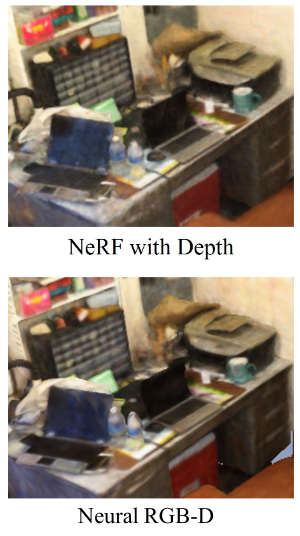
\includegraphics[width=0.5\textwidth]{undergraduate-thesis/images/related-work/neural-rgbd comparison with NeRF.png}
    \caption{直接将NeRF方法添加深度监督损失函数不能解决形状-辐射二义性。}
    \label{fig:related-work neural-rgbd comparison with NeRF}
\end{figure}

\subsection{多元传感信息融合}
虽然混合隐式表达在学习复杂场景信息时以及能在准确性上得到很大的提升,然而对于特征较少的墙面、纹理重复的表面,基于纯视觉的场景表示的精度仍然较差,一个直接的想法是使用深度传感器\cite{zabatani_intel_2020}引入深度输入作为额外的传感信号,然而直接在隐式场上添加深度监督信号会导致退化的结果(图\ref{fig:related-work neural-rgbd comparison with NeRF})。

NeuralRGB-D 是第一个将深度输入用于混合隐式表达优化的工作\cite{azinovic_neural_2022},作者使用了一个较为简单的用于体积渲染的混合隐式场方案:
\begin{equation}
    w_i = \mathtt{sigmoid}\left(\frac{f_{TSDF}(t)}{\mathtt{trunc}}\right)\cdot\mathtt{sigmoid}\left(-\frac{f_{TSDF}(t)}{\mathtt{trunc}}\right),
\end{equation}
其中$\mathtt{trunc}$为截断距离,通过加入这一超参数,使得原有的隐式符号距离场变为了一个隐式截断符号距离场,在自由空间内的距离值被设为截断距离。

\begin{figure}[htbp]
    \centering
    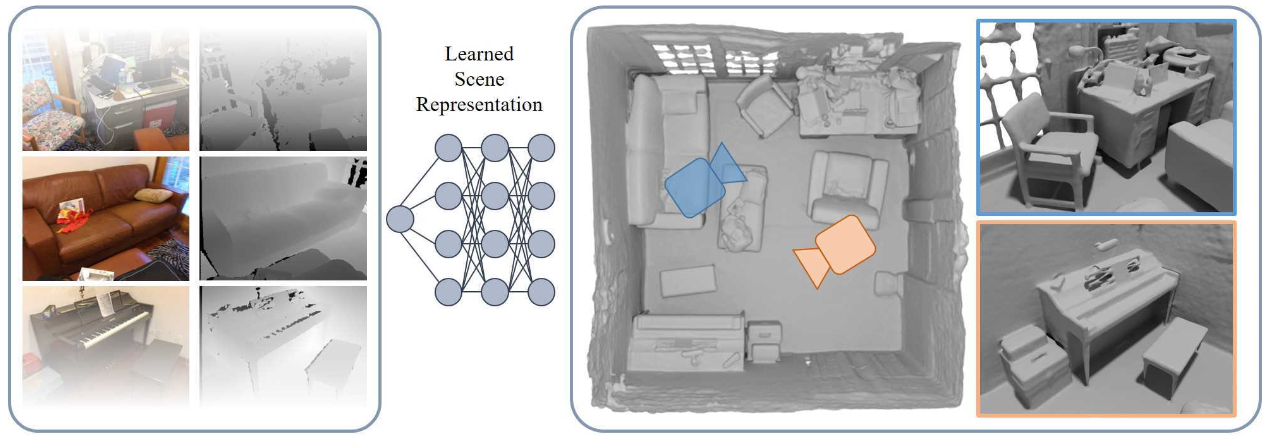
\includegraphics[width=\textwidth]{undergraduate-thesis/images/related-work/neural-rgbd problem.png}
    \caption{使用RGB-D多元信息优化隐式场的整体流程}
    \label{fig:related-work neural-rgbd formulation}
\end{figure}

本文将在第\ref{sec: related-work SDF optimization}节中介绍该方法的优化过程。通过引入深度监督,NeuralRGB-D可以获得可信的场景表面,通过混合隐式表征的加入,减弱形状-辐射二义性对于场景表示学习的影响。

\subsection{优化混合隐式场景表示}
当只需要优化神经辐射场时,大部分方法仅使用光度误差(公式\ref{eq: related-work photometric loss})即可得到较好的优化结果,然而当我们组合不同的隐式场时,原先的单目标优化过程演变成为了一个多目标的优化过程,这对损失函数的设计带来了挑战,在本节中,我们介绍优化隐式场的几种常用损失函数。
\begin{equation}
    \mathcal{L}_{color} = \sum_r||C(r)-\hat{C}(r)||_2^2
    \label{eq: related-work photometric loss}
\end{equation}

\subsubsection{距离场优化}
\label{sec: related-work SDF optimization}
注意到符号距离场编码了一个隐式表面,其梯度则代表了任意空间点到达其最近曲面的最速接近方向,因此NeuS\cite{wang_neus_2021}使用了Eikonal约束来限制距离场梯度向量趋近于单位方向向量:
\begin{equation}
    \mathcal{L}_{eikonal} = \sum_p(||\nabla f_{SDF}(p)||_2-1)^2
\end{equation}

对于截断的符号距离场\cite{azinovic_neural_2022},通常需要对场景的不同部分单独使用损失函数。在自由空间中,距离函数被截断,优化这部分距离场函数只需对网络输出的距离函数添加到截断距离$\mathtt{trunc}$的MSE损失函数:
\begin{equation}
    \mathcal{L}_{fs} = \sum_{p_{fs}}(f_{TSDF}(p_{fs})-\mathtt{trunc})^2
\end{equation}

而当空间点处于表面附近时($f_{TSDF}(p) \leq \mathtt{trunc}$)则需要根据输入深度估计该点的截断距离值,并使网络输出接近预测的截断距离:
\begin{equation}
    \mathcal{L}_{tr} = \sum_{p_{tr}}(f_{TSDF}(p_{tr})+t_{tr}-D)^2,
\end{equation}
$t_{tr}$为p点的归一化射线深度。

使用深度信息作为额外监督信号时,传统方案是直接使用网络预测深度与传感深度进行比较,使用MSE损失函数优化隐式表征:
\begin{equation}
    \mathcal{L}_{depth}=\sum_r||D(r)-\hat{D}(r)||_2^2
\end{equation}

然而由于深度传感器本身存在较大误差,直接用传感器输入值作为真实值存在一定问题,在DS-NeRF\cite{deng_depth-supervised_2022}使用KL散度使网络预测深度接近观测深度附近的一个高斯分布$\mathcal{N}(D, \hat{\sigma})$:
\begin{equation}
    \mathcal{L}_{DS-NeRF} = \sum\text{KL}[\mathcal{N}(D,\hat{\sigma}) | \hat{D}(r)]
\end{equation}

\begin{figure}[ht]
    \centering
    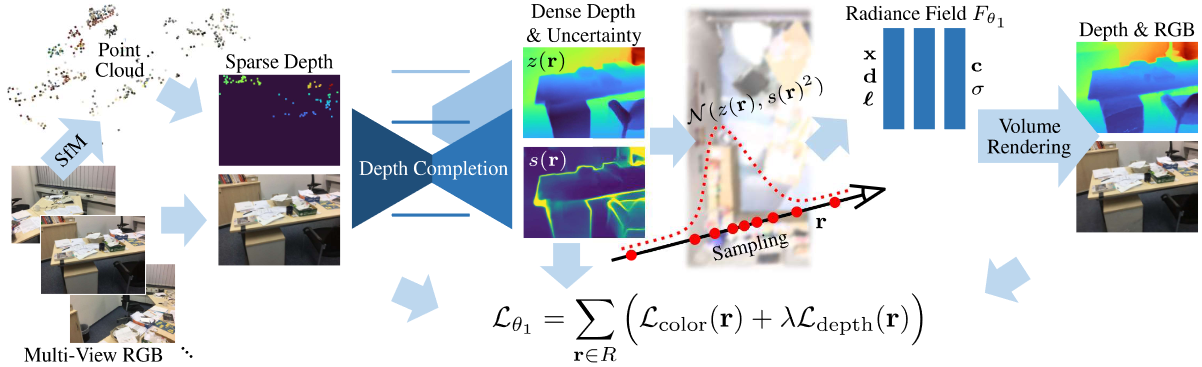
\includegraphics[width=\textwidth]{undergraduate-thesis/images/related-work/dense-depth prior.png}
    \caption{Dense Depth Prior\cite{roessle_dense_2022}中提出使用COLMAP\cite{schonberger_structure--motion_2016}稀疏点云补全后的深度作为监督信号,并引入基于不确定性的深度监督。}
    \label{fig:related-work dense depth prior}
\end{figure}

在Dense Depth Prior\cite{roessle_dense_2022}中,作者通过引入COLMAP\cite{schonberger_structure--motion_2016}稀疏点云,使用现成深度补全网络得到的深度图作为监督信号,这样生成的深度图相比深度传感器的噪声问题更加严峻,为了弥补真实深度精度的不足,作者引入了基于不确定性的深度损失函数:
\begin{equation}
    \mathcal{L}_{dense-depth}=\sum_r\left(\log(\hat{s}(r)^2)+\frac{(\hat{D}(r)-D(r))^2}{\hat{s}(r)^2}\right)
\end{equation}

\noindent\textbf{小结:} 本节介绍了为了建模精准的颜色和几何所使用的一系列距离-辐射混合隐式场景表达的基本概念和理论。距离-辐射场这一方向许多方法仍不成熟,从而存在诸多理论上的缺陷,本文将对现有方法中存在的两个误差进行分析,并提出解决方案。

\section{本章小结}
本章介绍了混合隐式表征这一新兴领域的相关理论基础。在本文的后几个章节中,将基于这些基础理论,并结合高质量渲染等隐式场理论,提出了一个新型混合隐式场景表示,并在真实世界数据中解决了一系列问题。